\section{Multiprojekt}

% % %
% GIRAF
% % %
\subsection{GIRAF}

\begin{frame}
\frametitle{Filosofi}

\begin{itemize}
\item \textit{Graphical Interface for Autistic Folk} (GIRAF)
\item Ét samlet værktøj med mange funktioner
\item Skal gøre livet nemmere for personer med autisme, samt deres forældre/pædagoger
\item (Skal fungere som institutioners eneste værktøj, derved også administration)
\end{itemize}

\end{frame}

\begin{frame}
\frametitle{Opbygning}

\begin{itemize}
\item Launcher (GIRAF)
\begin{itemize}
\item QR-kode pr. profil
\item 2 tilstande (Citizen eller Guardian)
\item Tilpasning til den enkelte profil
\begin{itemize}
\item Valg af applikationer
\item Indstillinger for applikationer
\end{itemize}
\end{itemize}
\item Applikationer
\begin{itemize}
\item Praktiske (e.g. PictoOplæser, Sekvens, Timer)
\item Administrative (Administration -- findes også som web-app)
\item Læring (Stemmespillet, Kategorispillet)
\end{itemize}
\end{itemize}

\end{frame}

\begin{frame}
\frametitle{Kunden}

\begin{itemize}
\item 6 kunder
\begin{itemize}
\item 4 pædagoger fra Birken
\item 1 pædagog fra ?
\item 1 talepædagog, tilknyttet Aalborg Kommune
\end{itemize}
\item Primær kunde
\begin{itemize}
\item Talepædagog (grundet Stemmespillet)
\end{itemize}
\end{itemize}

\end{frame}

% % %
% ORGANISATION
% % %
\subsection{Organisation}

\begin{frame}
\frametitle{Opbygning}

\begin{itemize}
\item Scrum of scrums
\begin{itemize}
\item 16 grupper
\item (1 statusgruppe)
\item 4 sprints
\end{itemize}
\end{itemize}

\centering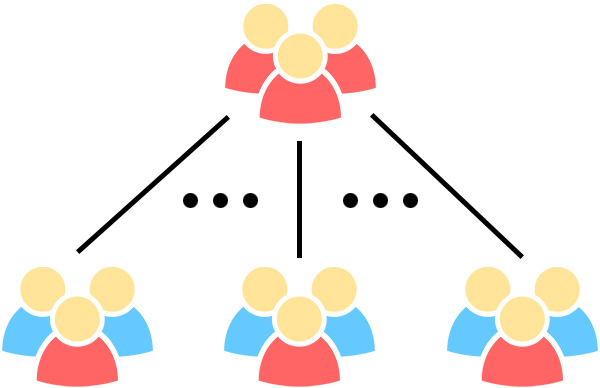
\includegraphics[height=.5\textheight]{pgraphics/scrum-of-scrums}

\end{frame}

\begin{frame}
\frametitle{Møder}

\begin{itemize}
\item Ugentlige statusmøder
\item Fælles sprint review
\item (Fælles) sprint planning
\end{itemize}

\end{frame}

\begin{frame}
\frametitle{Samarbejde}

\begin{itemize}
\item Fælles komponenter
\begin{itemize}
\item Database (OasisLib)
\item GUI (giraf-components)
\item (Mindre dele)
\end{itemize}
\item Værktøjer
\begin{itemize}
\item Redmine
\item Git
\item Jenkins
\end{itemize}
\item Specialister
\end{itemize}

\end{frame}

% % %
% CARS
% % %
\subsection{Cars}

\begin{frame}
\frametitle{Filosofi}

\end{frame}

\begin{frame}
\frametitle{Udvikling}

\end{frame}

\begin{frame}
\frametitle{Fremgangsmåde}

\end{frame}